\documentclass[compress]{beamer}
\setbeamercolor{normal text}{fg=white}
\setbeamercovered{transparent, still covered={\opaqueness<1->{0}}, again covered={\opaqueness<1->{30}}}
\beamertemplatesolidbackgroundcolor{black}
\usecolortheme[named=white]{structure} 
\usepackage{caption}
\captionsetup{labelformat=empty}
\setbeamertemplate{navigation symbols}{} 
%\usefonttheme{structurebold}
\usepackage{listings}
\usepackage{ulem}
\usepackage[scaled]{helvet}
\renewcommand*\familydefault{\sfdefault} %% Only if the base font of the document is to be sans serif
\usepackage[T1]{fontenc}
\usepackage{setspace}
%\usepackage{beamerthemesplit}
\usepackage{graphics}
\usepackage{hyperref}
\usepackage{graphicx}
\usepackage{verbatim}
\usepackage{amssymb}
\usepackage{wrapfig}
\usefonttheme[onlymath]{serif}
\usepackage{cmbright}

\def\labelitemi{\textemdash}
\setbeamertemplate{frametitle}{
	\begin{centering}
		\vskip15pt
		\insertframetitle
		\par
	\end{centering}
} 
\title[Names]{\\ \vspace{10mm} pwned: exposure from data breaches}
\author[Sood and Laohaprapanon]{gaurav and ken}
  \large
\date[2019]{}
\subject{Paper}
\begin{document}
\newcommand{\multilineR}[1]{\begin{tabular}[b]{@{}r@{}}#1\end{tabular}}
\newcommand{\multilineL}[1]{\begin{tabular}[b]{@{}l@{}}#1\end{tabular}}
\newcommand{\multilineC}[1]{\begin{tabular}[b]{@{}c@{}}#1\end{tabular}}
\newcommand{\indep}{\rotatebox[origin=c]{90}{$\models$}}
\newenvironment{large_enum}{
\Large
\begin{itemize}
  \setlength{\itemsep}{7pt}
  \setlength{\parskip}{0pt}
  \setlength{\parsep}{0pt}
}{\end{itemize}}

\begin{comment}

setwd(paste0(githubdir, "pwned_dev/present/"))
tools::texi2dvi("pwned.tex", pdf = TRUE, clean = TRUE)
setwd(githubdir)

\end{comment}
  \frame
  {
    \titlepage
  }

\frame{
\begin{center}
\Large{the price of a data breach}
\end{center}
}

\frame{
\begin{large_enum}
	\item[-]<1-6>\normalsize{\texttt{September 22, 2016}}
    \item[]<2-6>\normalsize{\textit{Yahoo!} reveals that \alert<6>{500M} accounts have been compromised.}
	\item[-]<3-6>\normalsize{\texttt{December 14, 2016}}
	\item[]<4-6>\normalsize{\textit{Yahoo!} announces that data had been stolen from nearly \alert<6>{1 billion} user accounts in a different breach.}
	\item[-]<5-6>\normalsize{Verizon, in the middle of negotiating a takeover of \textit{Yahoo!}, values the breaches at \$350M, less than a \alert<6>{quarter-cent per breached account}.}
	\item[-]<7>\normalsize{\texttt{October 4, 2017}}
	\item[]<8>\normalsize{\textit{Yahoo!} revises the estimate for the latter breach to 3 billion.}
\end{large_enum}
}


\frame{
\begin{center}
\Large{the consequence of a low price of a breach}
\end{center}
}

\frame{
\Large{Data\\}
\begin{large_enum}
   \item[-]<1-3> YouGov
		\begin{enumerate}
			\item[-]<2-> $n = 5,000$
			\item[-]<3-> Matched sampling. Median Error is 1\%.
	    \end{enumerate}
	   \end{large_enum}
	\pause
}

\frame{
\begin{table}[!htb]
\centering
\caption{Comparison Between YouGov and CPS 2018} 
\label{table:cps_yg}
\begingroup\small
\begin{tabular}{lrrr}
  \hline
 & cps & yg & diff \\ 
  \hline
Age &  &  &  \\ 
  18 to 25 & 0.14 & 0.13 & \alert<1>{0.01} \\ 
  26 to 35 & 0.18 & 0.18 & \alert<1>{0.00} \\ 
  36 to 50 & 0.25 & 0.23 & \alert<1>{0.02} \\ 
  51 to 65 & 0.25 & 0.26 & \alert<1>{-0.01} \\ 
  66 to 80+ & 0.19 & 0.18 & \alert<1>{0.01} \\ 
  & & &  \\ 
  Sex &  &  &  \\ 
  Male & 0.48 & 0.51 & \alert<1>{-0.03} \\ 
  Female & 0.52 & 0.49 & \alert<1>{0.03} \\ 
\hline
\end{tabular}
\endgroup
\end{table}


}

\frame{
\begin{table}[!htb]
\centering
\caption{Comparison Between YouGov and CPS 2018} 
\label{table:cps_yg}
\begingroup\small
\begin{tabular}{lrrr}
  \hline
 & cps & yg & diff \\ 
  \hline

  Race &  &  &  \\ 
  White alone & 0.78 & 0.64 & \alert<1>{0.14} \\ 
  Black or African American alone & 0.13 & 0.12 & \alert<1>{0.01} \\ 
  American Indian and Alaska Native alone & 0.01 & 0.01 & \alert<1>{0.00}\\ 
   &  &  &  \\ 

  Educational Attainment &  &  &  \\ 
  No high school diploma & 0.11 & 0.07 & \alert<1>{0.04}\\ 
  High school or equivalent & 0.29 & 0.33 & \alert<1>{-0.04}\\ 
  Some college, less than 4-yr degree & 0.28 & 0.31 & \alert<1>{-0.03}\\ 
  Bachelor's degree or higher & 0.32 & 0.29 & \alert<1>{0.03}\\ 
\hline
\end{tabular}
\endgroup
\end{table}
}

\frame{
\Large{Data\\}
\begin{large_enum}
   \item[-]<0> YouGov
		\begin{enumerate}
			\item[-]<0-> $n = 5,000$
			\item[-]<0-> Matched sampling. Median Error is 1\%.
	    \end{enumerate}
	    
	\item[-]<2-5>Have I Been Pwned (HIBP):
		\begin{enumerate}
			\item[-]<3->Clearinghouse of information about data breaches
			\item[-]<4->It currently carries data from 293 breaches covering 278 unique domains
			\item[-]<5->Information about 5,235,843,322 breached accounts
		\end{enumerate}
	\item[-]<6>Query HIBP with the email ID on the file.
	\end{large_enum}

\only<7->{\Large{Empirical Caveat\\}}
\begin{large_enum}
	\item[-]<8->Most breaches are never discovered
	\item[-]<9>We can only estimate the \textit{lower bound}.
\end{large_enum}
}

\frame{
\frametitle{The horror! The horror!}
\begin{large_enum}
	\item[-]<2->\alert<5>{14,979} breaches are associated with the 5,000 emails on file. 
	\item[-]<3->Or on average, there are \alert<5>{three breaches per person}. The median is also three. 
	\item[-]<4->And at least \alert<5>{82.84\%} of Americans' accounts have been breached at least once. 
\end{large_enum}
}

\frame{
\begin{center}
	\Large{who is pwned?}
\end{center}
}

\frame{
	\only<1>{\Large{the age of the pwned}}

\pause
\only<2>{
\begin{figure}[H]
\centering
	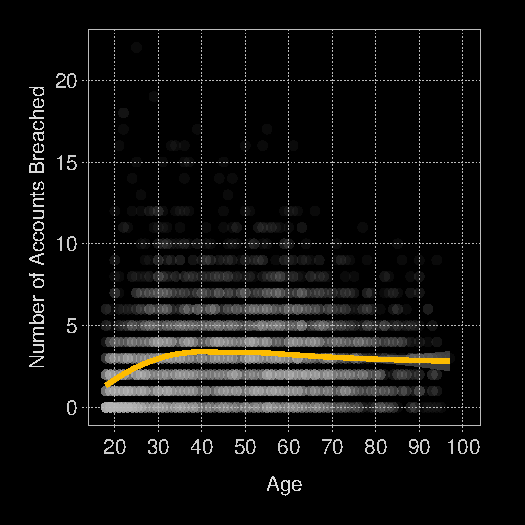
\includegraphics[scale = 1]{../figs/age_pwned_present.pdf}
\end{figure}
}
}

\frame{
\scriptsize

% Table created by stargazer v.5.2.2 by Marek Hlavac, Harvard University. E-mail: hlavac at fas.harvard.edu
% Date and time: Mon, Feb 11, 2019 - 7:51:27 PM
\begin{table}[!htbp] \centering 
  \caption{Number of Breaches by Age} 
  \label{} 
\begin{tabular}{@{\extracolsep{5pt}}lc} 
\\[-1.8ex]\hline 
\hline \\[-1.8ex] 
 & \multicolumn{1}{c}{\textit{Dependent variable:}} \\ 
\cline{2-2} 
\\[-1.8ex] & Number of Breaches \\ 
\hline \\[-1.8ex] 
 ns(age, 2)1 & 2.23$^{***}$ \\ 
  & (.20) \\ 
  ns(age, 2)2 & $-$.90$^{***}$ \\ 
  & (.21) \\ 
  Constant & 2.01$^{***}$ \\ 
  & (.09) \\ 
 \hline \\[-1.8ex] 
Observations & 5,000 \\ 
R$^{2}$ & .03 \\ 
Adjusted R$^{2}$ & .03 \\ 
\hline 
\hline \\[-1.8ex] 
\textit{Note:}  & \multicolumn{1}{r}{$^{*}$p$<$0.1; $^{**}$p$<$0.05; $^{***}$p$<$0.01} \\ 
\end{tabular} 
\end{table} 

}

\frame{
	\only<1>{\Large{the race of the pwned}}

\pause
\only<2>{

\begin{figure}[H]
  \centering
   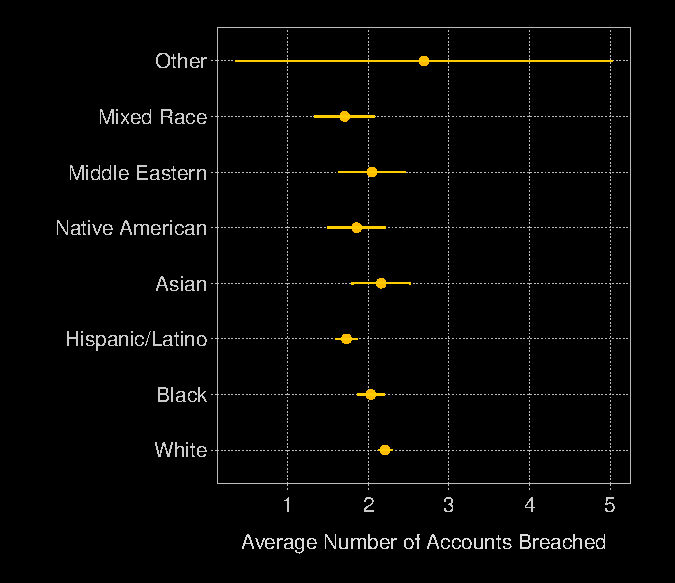
\includegraphics[scale = .85]{../figs/race_pwned_present.pdf}
\end{figure}
}
}

\frame{
\vspace{-.4cm}
\scriptsize{
	
% Table created by stargazer v.5.2.2 by Marek Hlavac, Harvard University. E-mail: hlavac at fas.harvard.edu
% Date and time: Sat, Apr 27, 2019 - 5:55:59 PM
\begin{table}[!htbp] \centering 
  \caption{Number of Breaches by Race/Ethnicity} 
  \label{tab:race_breaches} 
\begin{tabular}{@{\extracolsep{5pt}}lc} 
\\[-1.8ex]\hline 
\hline \\[-1.8ex] 
 & \multicolumn{1}{c}{\textit{Dependent variable:}} \\ 
\cline{2-2} 
\\[-1.8ex] & Number of Breaches \\ 
\hline \\[-1.8ex] 
 Black & .04 \\ 
  & (.12) \\ 
  Hispanic/Latino & $-$.62$^{***}$ \\ 
  & (.10) \\ 
  Asian & $-$.30 \\ 
  & (.23) \\ 
  Native American & $-$.16 \\ 
  & (.36) \\ 
  Middle Eastern & $-$.46$^{**}$ \\ 
  & (.24) \\ 
  Mixed Race & $-$.67$^{**}$ \\ 
  & (.29) \\ 
  Other & $-$.20 \\ 
  & (.73) \\ 
  Constant & 3.12$^{***}$ \\ 
  & (.05) \\ 
 \hline \\[-1.8ex] 
Observations & 5,000 \\ 
R$^{2}$ & .01 \\ 
Adjusted R$^{2}$ & .01 \\ 
\hline 
\hline \\[-1.8ex] 
\textit{Note:}  & \multicolumn{1}{r}{$^{*}$p$<$0.1; $^{**}$p$<$0.05; $^{***}$p$<$0.01} \\ 
\end{tabular} 
\end{table} 

}
}

\frame{
	\only<1>{\Large{the sex of the pwned}}

\pause
\only<2>{

\begin{figure}[H]
  \centering
   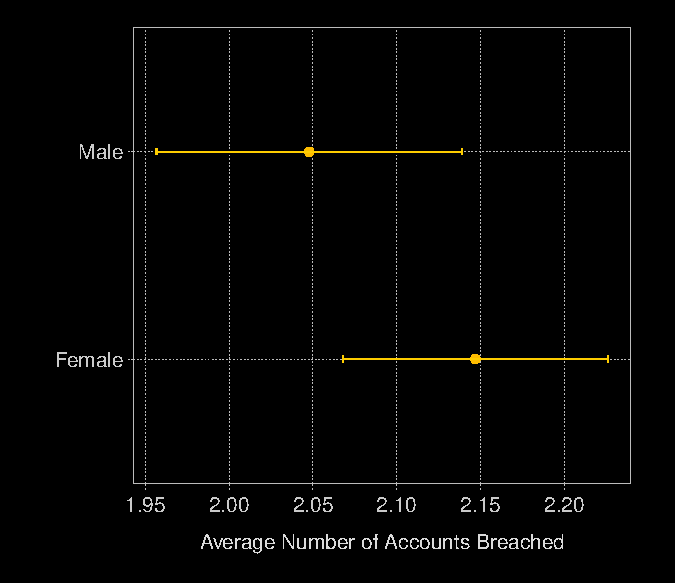
\includegraphics[scale = .85]{../figs/sex_pwned_present.pdf}
\end{figure}
}
}

\frame{
\scriptsize

% Table created by stargazer v.5.2.2 by Marek Hlavac, Harvard University. E-mail: hlavac at fas.harvard.edu
% Date and time: Sun, Feb 17, 2019 - 2:48:10 PM
\begin{table}[!htbp] \centering 
  \caption{Number of Breaches by Sex} 
  \label{} 
\begin{tabular}{@{\extracolsep{5pt}}lc} 
\\[-1.8ex]\hline 
\hline \\[-1.8ex] 
 & \multicolumn{1}{c}{\textit{Dependent variable:}} \\ 
\cline{2-2} 
\\[-1.8ex] & Number of Breaches \\ 
\hline \\[-1.8ex] 
 Male & $-$.35$^{***}$ \\ 
  & (.07) \\ 
  Constant & 3.17$^{***}$ \\ 
  & (.05) \\ 
 \hline \\[-1.8ex] 
Observations & 5,000 \\ 
R$^{2}$ & .004 \\ 
Adjusted R$^{2}$ & .004 \\ 
\hline 
\hline \\[-1.8ex] 
\textit{Note:}  & \multicolumn{1}{r}{$^{*}$p$<$0.1; $^{**}$p$<$0.05; $^{***}$p$<$0.01} \\ 
\end{tabular} 
\end{table} 

}

\frame{
	\only<1>{\Large{the education of the pwned}}

\pause
\only<2>{

\begin{figure}[H]
  \centering
    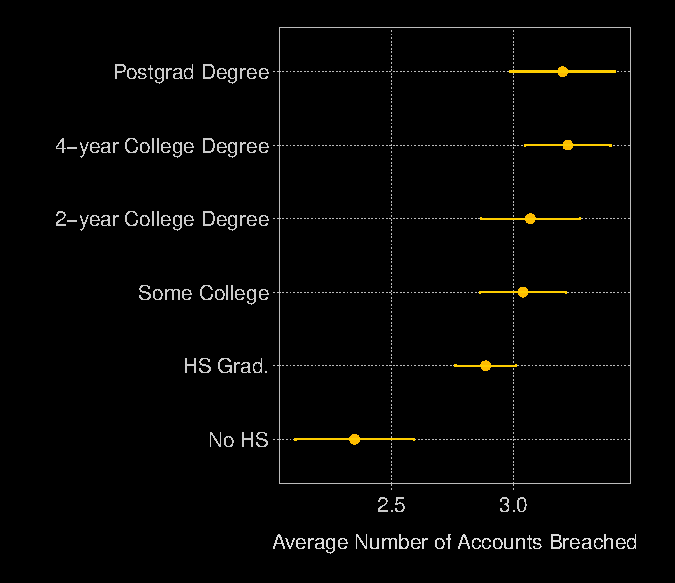
\includegraphics[scale = .9]{../figs/educ_pwned_present.pdf}
\end{figure}
}
}

\frame{
\scriptsize

% Table created by stargazer v.5.2.2 by Marek Hlavac, Harvard University. E-mail: hlavac at fas.harvard.edu
% Date and time: Sat, Apr 27, 2019 - 5:55:59 PM
\begin{table}[!htbp] \centering 
  \caption{Number of Breaches by Education} 
  \label{tab:educ_breaches} 
\begin{tabular}{@{\extracolsep{5pt}}lc} 
\\[-1.8ex]\hline 
\hline \\[-1.8ex] 
 & \multicolumn{1}{c}{\textit{Dependent variable:}} \\ 
\cline{2-2} 
\\[-1.8ex] & Number of Breaches \\ 
\hline \\[-1.8ex] 
 HS Grad. & .54$^{***}$ \\ 
  & (.16) \\ 
  Some College & .69$^{***}$ \\ 
  & (.16) \\ 
  2-year College Degree & .72$^{***}$ \\ 
  & (.18) \\ 
  4-year College Degree & .87$^{***}$ \\ 
  & (.17) \\ 
  Postgrad Degree & .85$^{***}$ \\ 
  & (.18) \\ 
  Constant & 2.35$^{***}$ \\ 
  & (.14) \\ 
 \hline \\[-1.8ex] 
Observations & 5,000 \\ 
R$^{2}$ & .01 \\ 
Adjusted R$^{2}$ & .01 \\ 
\hline 
\hline \\[-1.8ex] 
\textit{Note:}  & \multicolumn{1}{r}{$^{*}$p$<$0.1; $^{**}$p$<$0.05; $^{***}$p$<$0.01} \\ 
\end{tabular} 
\end{table} 

}

\frame{
\begin{center}
	\only<1>{\Large{who is most at blame?}}
	\Large{\only<2>{or most frequently implicated domains}}

\end{center}
}
\frame{
\begin{table}[h!]
\centering
\scriptsize
\begin{tabular}{ l c }
\hline    
domain name & n \\
\hline
\alert<3>{rivercitymediaonline.com} &   2,913 \\
\alert<2>{linkedin.com}             &   1,089 \\
modbsolutions.com        &   1,067\\
\alert<2>{myspace.com}              &   1,059\\
data4marketers.com       &    996\\
cashcrate.com            &    856\\
\alert<2>{adobe.com}                &    609\\
disqus.com               &    570\\
ticketfly.com            &    393\\
\alert<2>{tumblr.com}               &    340\\
\alert<2>{dropbox.com}              &    288\\
dailymotion.com          &    255\\
last.fm                  &    248\\
evony.com                &    171\\
clixsense.com            &    150\\
cafemom.com              &    145\\
imesh.com                &    144\\
kickstarter.com          &    140\\
edmodo.com               &    130\\
zomato.com               &    112\\
neopets.com              &    108\\
\hline
\end{tabular}
\label{table:domain_dat}
\end{table}
}


\frame{
\Large{Upshot}
\begin{large_enum}
	\item[-]<2>at least 82.84\% of Americans' accounts have been breached at least once
	\item[-]<3>people who use online services more are somewhat more likely to have their accounts breached
	\item[-]<4>popular websites are to blame!
	\end{large_enum}
}

\frame{
	\begin{center}
		\Large{thank you!\\\vspace{15mm}}
		\normalsize{Data and scripts at:\\ \href{https://github.com/themains/pwned/}{https://github.com/themains/pwned/}}
	\end{center}
}
\frame{
\begin{center}
	\only<1>{\Large{exposure to the worst case}}
	\only<2>{counting only verified, non-spamlist breaches.}
\end{center}
}

\frame{
\scriptsize
\begin{table}[!htb]
\centering
\begingroup\small
\begin{tabular}{lrr}
  \hline
 & mean & se \\ 
  \hline
Age &  &  \\ 
  (18,25] & 1.63 & 0.10 \\ 
  (25,35] & 2.44 & 0.08 \\ 
  (35,50] & 2.37 & 0.07 \\ 
  (50,65] & 2.16 & 0.06 \\ 
  (65,100] & 1.78 & 0.05 \\ 
  Missing & 0.91 & 0.13 \\ 
   &  &  \\ 
  Education &  &  \\ 
  No HS & 1.53 & 0.09 \\ 
  HS Grad. & 1.91 & 0.05 \\ 
  Some College & 2.22 & 0.08 \\ 
  2-year College Degree & 2.10 & 0.08 \\ 
  4-year College Degree & 2.37 & 0.08 \\ 
  Postgrad Degree & 2.30 & 0.08 \\ 
\hline
\end{tabular}
\endgroup
\end{table}
}

\frame{
\scriptsize
\begin{table}[!htb]
\centering
\begingroup\small
\begin{tabular}{lrr}
  \hline
 & mean & se \\ 
  \hline
  Sex &  &  \\ 
  Female & 2.15 & 0.04 \\ 
  Male & 2.05 & 0.05 \\ 
   &  &  \\ 
  Race &  &  \\ 
  White & 2.21 & 0.04 \\ 
  Black & 2.03 & 0.08 \\ 
  Hispanic/Latino & 1.73 & 0.07 \\ 
  Asian & 2.16 & 0.18 \\ 
  Native American & 1.85 & 0.18 \\ 
  Middle Eastern & 2.05 & 0.21 \\ 
  Mixed Race & 1.70 & 0.19 \\ 
  Other & 2.69 & 1.19 \\
\hline
\end{tabular}
\endgroup
\end{table}
}

\end{document}
